\documentclass[%
fontsize=11%
,a5paper%
,DIV=15%
]{scrartcl}
%scrartcl



\usepackage{gredocument}
\usepackage{adaptateur}
\usepackage{psaume}

\title{\centrer{\huge{Rituel du mariage}}}
\author{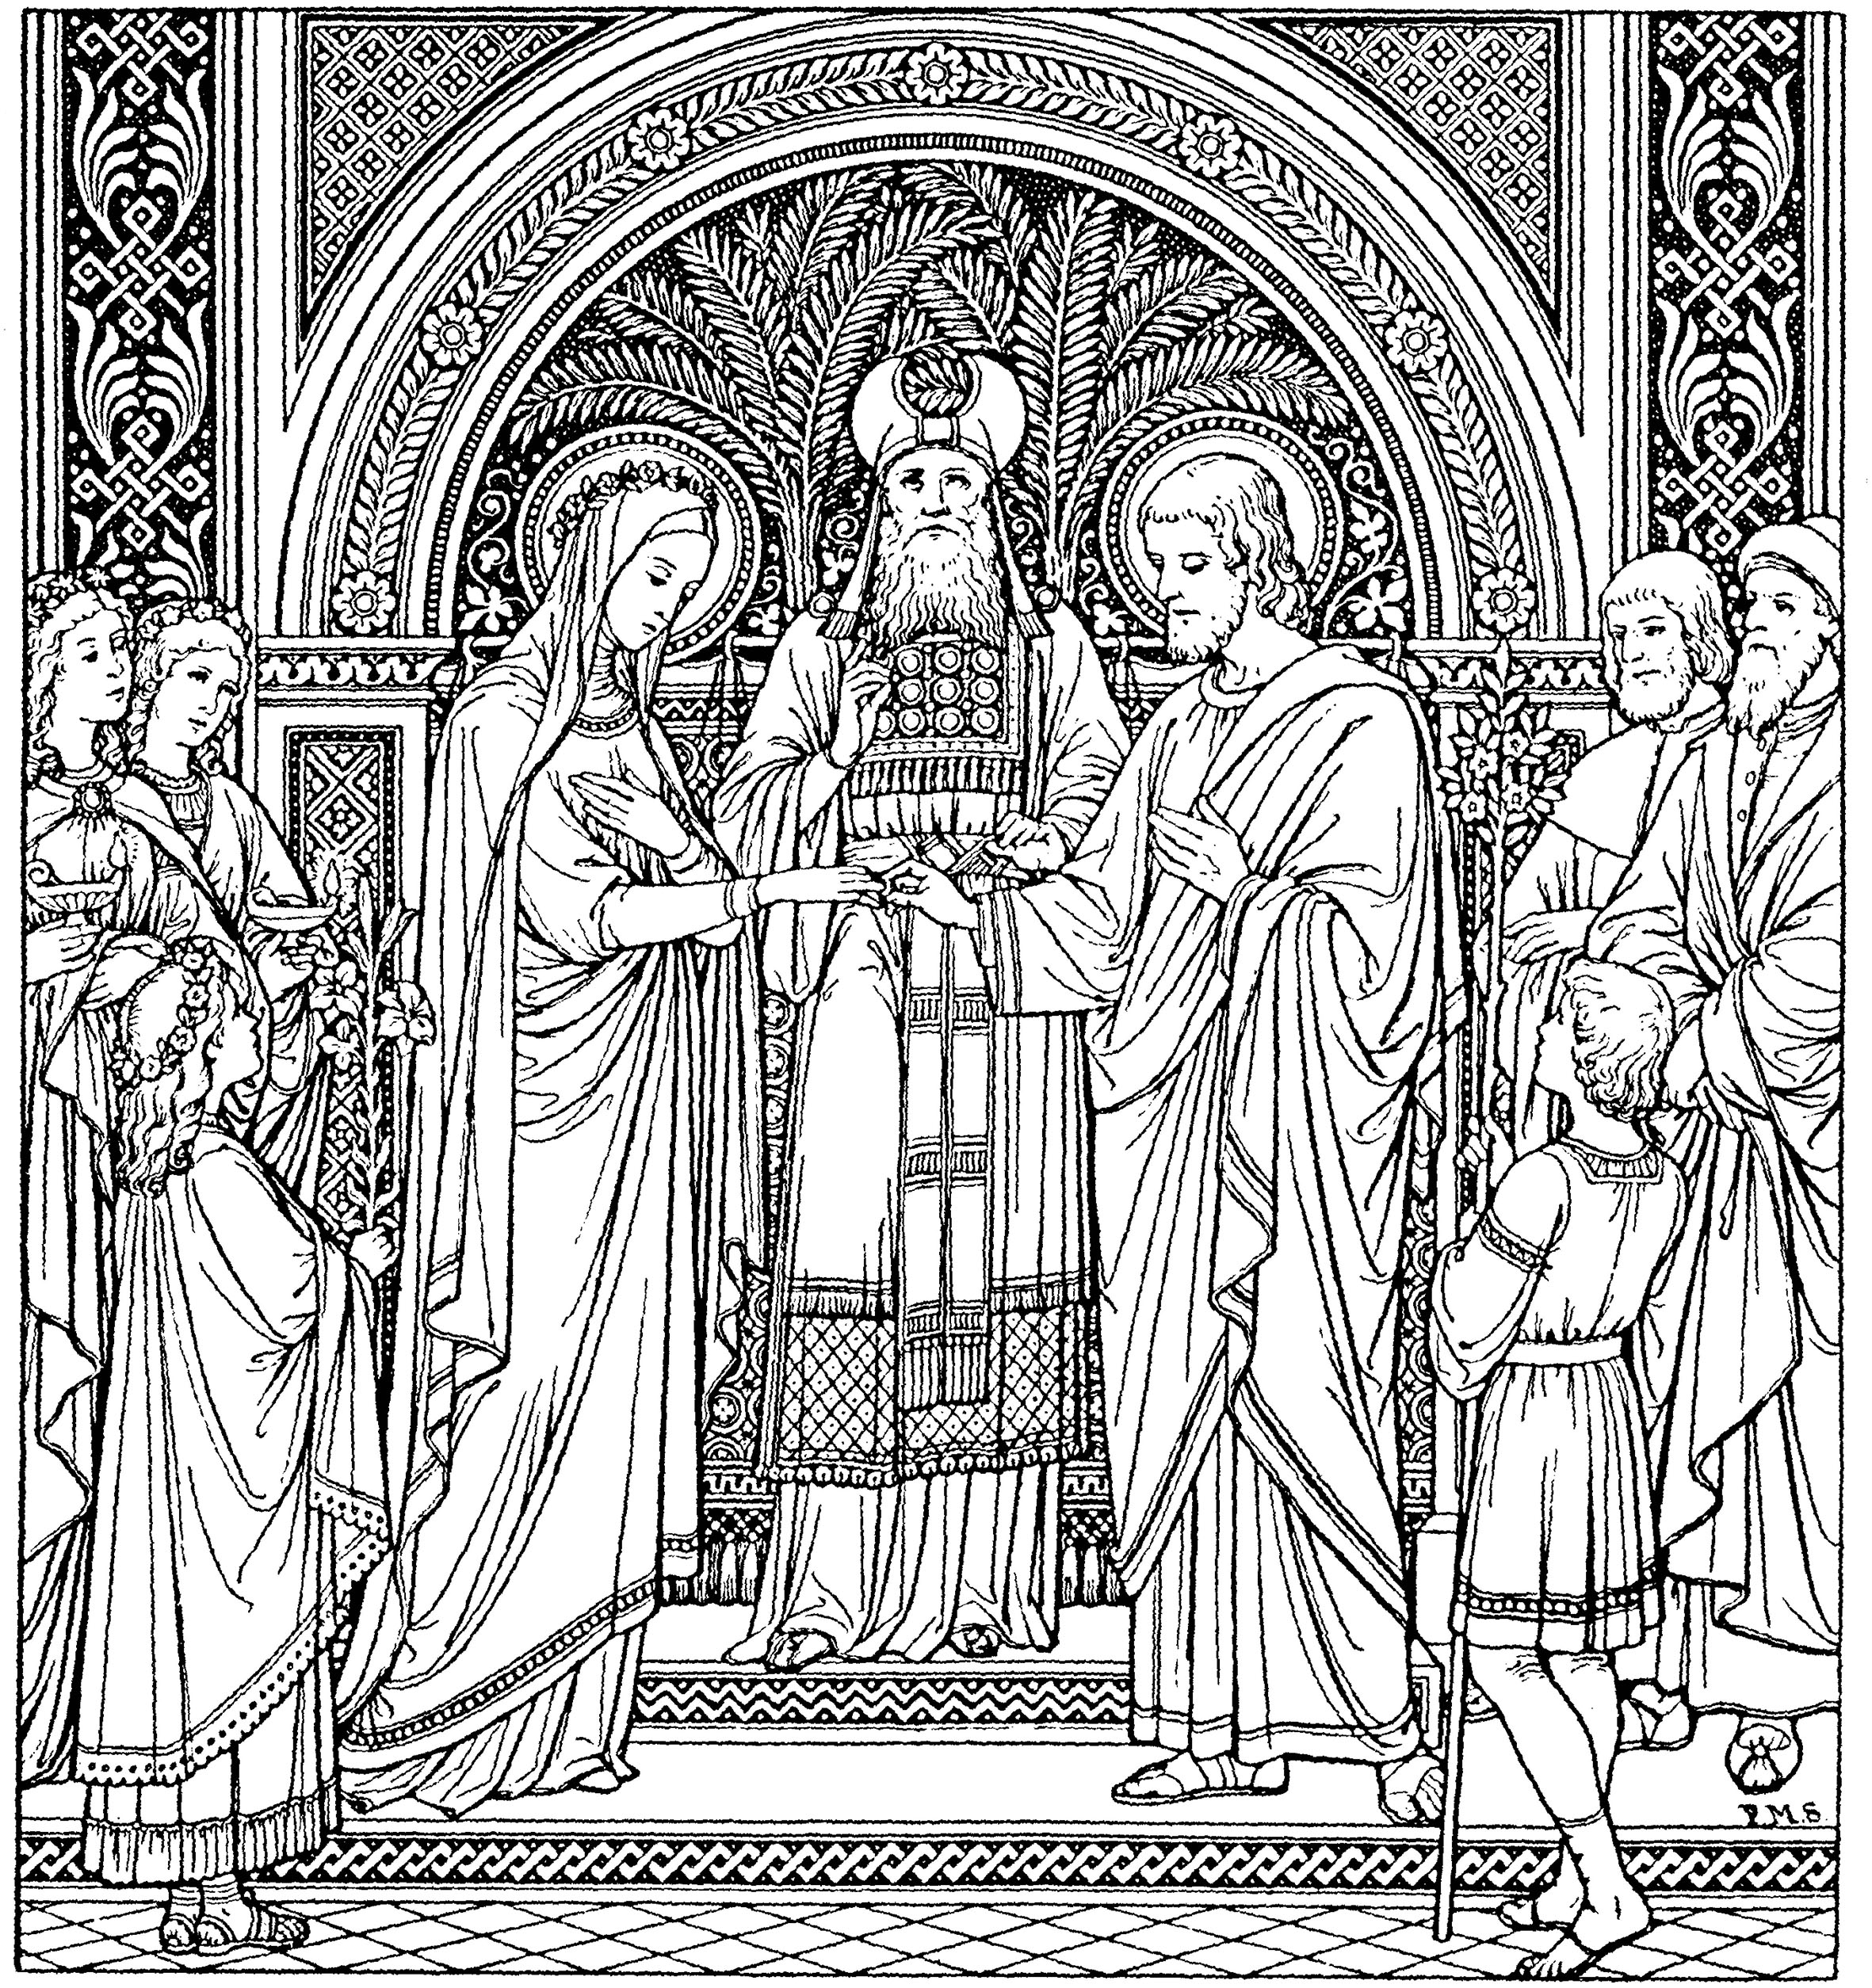
\includegraphics[height=12cm]{images/MariageVierge.jpg}}
\date{en dehors de la messe}

\makeindex
        \definecolor{rubrum}{rgb}{.6,0,0}
        \def\rubrum{\color{rubrum}}%%%%%%%mettre"\def\rubrum{\color{rubrum}}" pour avoir le texte adéquat en rouge
        \def\nigra{\color{black}}
            \redlines
            \definecolor{gregoriocolor}{rgb}{.6,0,0}
        %
        %\let\red\rubrum
        \newcommand{\rep}[2]{\versio{\R \textbf{#1}}{\R \textbf{#2}}}
        \newcommand{\vers}[2]{\versio{\V {#1}}{\V {#2}}}
        \newcommand{\enrouge}[1]{\rubrum{#1}\nigra{}}

%%%%%%%%%%%%%%%%%%%%%%%%%%%%%%%%%%%%%%%%%%%%%%%%%%%%%%%%%%%%%%%%%%%%%%%%%%%%%%%%%%%%%%%%%%%%%%%%%%%%
\begin{document}

\maketitle
\thispagestyle{empty}
%\pageblanche

        \newfontfamily\lettrines[Scale=1.3]{LettrinesPro800}
            \def\gretextformat#1{{\fontsize{\taillepolice}{\taillepolice}\selectfont #1}}
            \def\greinitialformat#1{{\lettrines #1}}
            
\titre{Les consentements}

\rubrique{Le prêtre s'adresse au fiancé :}

  \textsc{Monsieur \enrouge{N.}, voulez-vous prendre pour légitime épouse \enrouge{N.}, ici présente, selon le rite de notre mère la Sainte Eglise?}

\rubrique{Le fiancé répond : }  \textsc{Oui, je le veux.}

\rubrique{Puis, s'adressant à la fiancée :}

  \textsc{Mademoiselle \enrouge{N.}, voulez-vous prendre pour légitime époux \enrouge{N.}, ici présent, selon le rite de notre mère la Sainte Eglise?}

\rubrique{La fiancée répond : }  \textsc{Oui, je le veux.}

\vspace{2cm}
\rubrica{Le nouvel époux dit alors :}
Moi, \enrouge{N.N.} Je vous prends pour ma légitime épouse, afin de vous garder à partir de ce jour, pour le meilleur et pour le pire, à travers richesse et pauvreté, maladie et santé, jusqu'à ce que la mort nous sépare.

\rubrica{Et la nouvelle épouse :}
Moi, \enrouge{N.N.} Je vous prends pour mon légitime époux, afin de vous garder à partir de ce jour, pour le meilleur et pour le pire, à travers richesse et pauvreté, maladie et santé, jusqu'à ce que la mort nous sépare.

\rubrique{Le prêtre invite alors les époux à se donner la main droite. Puis il confirme l'engagement dont il vient d'être témoin en disant :}

\traduire{Ego conjungo vos in matrimonium, in nomine Patri, et Filii~\x\ et Spiritui Sancti. Amen.}{Je vous déclare unis par le mariage au nom du Père et du Fils~\x\ et du Saint Esprit. Ainsi soit-il.}

\vspace{0.5cm}
\titre{Bénédiction des Anneaux}

\rubrique{Le prêtre bénit les anneaux :}

\traduire{\V Adiutorium nostrum in nomine Domini.}{\V Notre secours est dans le nom du Seigneur.}

\traduire{\R \textbf{Qui fecit c\ae lum et terram.}}{\R \textbf{Qui a fait le ciel et la terre.}}


\traduire{%
\V~Dómine, exáudi oratiónem meam.}{%
\V~Seigneur, exaucez ma prière.}

\traduire{%
\R~\textbf{Et clamor meus ad te véniat.}}{%
\R~\textbf{Que mon appel vous parvienne.}}

\traduire{%
\V~Dóminus vobíscum.}{%
\V~Le Seigneur soit avec vous.}

\traduire{%
\R~\textbf{Et cum spíritu tuo.}}{%
\R~\textbf{Et avec votre esprit.}}

\traduire{%
Orémus.}{%
Prions.}

\traduire{ Bene~\x\ dic Domine annulos istos quos nos in tuo nomine bene~\x\ dicimus, ut qui eos gestaverint, fidelit\'a tem integram invicem tenentes, in pace et volunt\'a te tua perm\'a neant, atque in mutua caritate semper vivant. Per Christum.}{Béni~\x\ ssez, Seigneur, ces anneaux que nous béni~\x\ ssons en votre nom, afin que ceux qui les porteront, les conservent dans une fidélité entière, demeurent dans la paix et dans votre volonté, et qu'ils vivent toujours dans une mutuelle affection. Par le Christ Notre-Seigneur.}

\traduire{\R \textbf{Amen.}}{\R \textbf{Ainsi soit-il.}}

\rubrique{L'époux passe au doigt de son épouse et à son doigt l'anneau qui ne les quittera plus.
Le prêtre bénit ce geste et appelle les grâces divines sur l'union irrévocable qui vient de se conclure.}

\titre{Prière pour les époux}

\vspace*{0.5cm}
\versio{In nomine Patris~\x\ et Filii, et Spiritu Sancti. Amen.
}{Au nom du Père~\x\ et du Fils et du Saint-Esprit. Ainsi soit-il.}
\versio{\V Confirma hoc, Deus, quod operatus est in nobis.
}{\V Confirmez, Seigneur, ce que vous avez accompli en nous.}

\versio{\R \textbf{ A templo sancto tuo, quod est in Jerusalem.}
}{\R \textbf{De votre saint temple, en Jérusalem.}}

\versio{Kyrie, eleison.
Christe, eleison.
Kyrie, eleison.
}{Seigneur, ayez pitié de nous.
Christ, ayez pitié de nous.
Seigneur, ayez pitié de nous.}

\versio{Pater noster... (secreto).
}{Notre Père... (à voix basse)}

\versio{\V Et ne nos inducas in tentationem.
}{\V Et ne nous laissez pas succomber à la tentation.}

\versio{\R \textbf{ Sed libera nos a malo.}
}{\R \textbf{Mais délivrez-nous du mal.}}

\versio{\V Salvos fac servos tuos.
}{\V Seigneur, sauvez vos serviteurs.}

\versio{\R \textbf{ Deus meus, sperantes in te.}
}{\R \textbf{Qui espèrent en vous, mon Dieu.}}

\versio{\V Mitte eis, Domine, auxilium de sancto.
}{\V Envoyez-leur votre aide, Seigneur, de votre sanctuaire.}

\versio{\R \textbf{ Et de Sion tuere eos.}
}{\R\textbf{ Et de Sion, soutenez-les.}}

\versio{\V Esto eis Domine, turris fortitudinis.
}{\V Soyez pour eux, Seigneur, comme une tour fortifiée.}

\versio{\R \textbf{ A facie inimici.}
}{\R \textbf{Dressée contre l'ennemi.}}

\versio{\V Domine exaudi orationem meam.
}{\V Seigneur, exaucez ma prière.}

\versio{\R \textbf{ Et clamor meus ad te veniat.}
}{\R \textbf{Et que mon appel monte jusqu'à vous.}}

\versio{\V Dominus vobiscum.
}{\V Le Seigneur soit avec vous.}

\versio{\R \textbf{ Et cum spiritu tuo.}
}{\R \textbf{Et avec votre esprit.}}

\versio{Oremus.\\
Respice, quæsumus, Domine, super hos famulos tuos, et institutis tuis quibus propagationem humani generis ordinasti, benignus assiste : ut qui te auctore junguntur, te auxiliante serventur. Per Christum Dominum nostrum
}{Prions\\
Jetez les yeux, Seigneur, sur ces époux vos serviteurs et protégez cette institution que vous avez établie pour la propagation du genre humain, afin qu'unis par vous ils soient également soutenus et gardés par votre secours. Par le Christ Notre-Seigneur.}

\versio{\R \textbf{Amen.}}{Ainsi soit-il}
\vspace{1cm}
\begin{center}
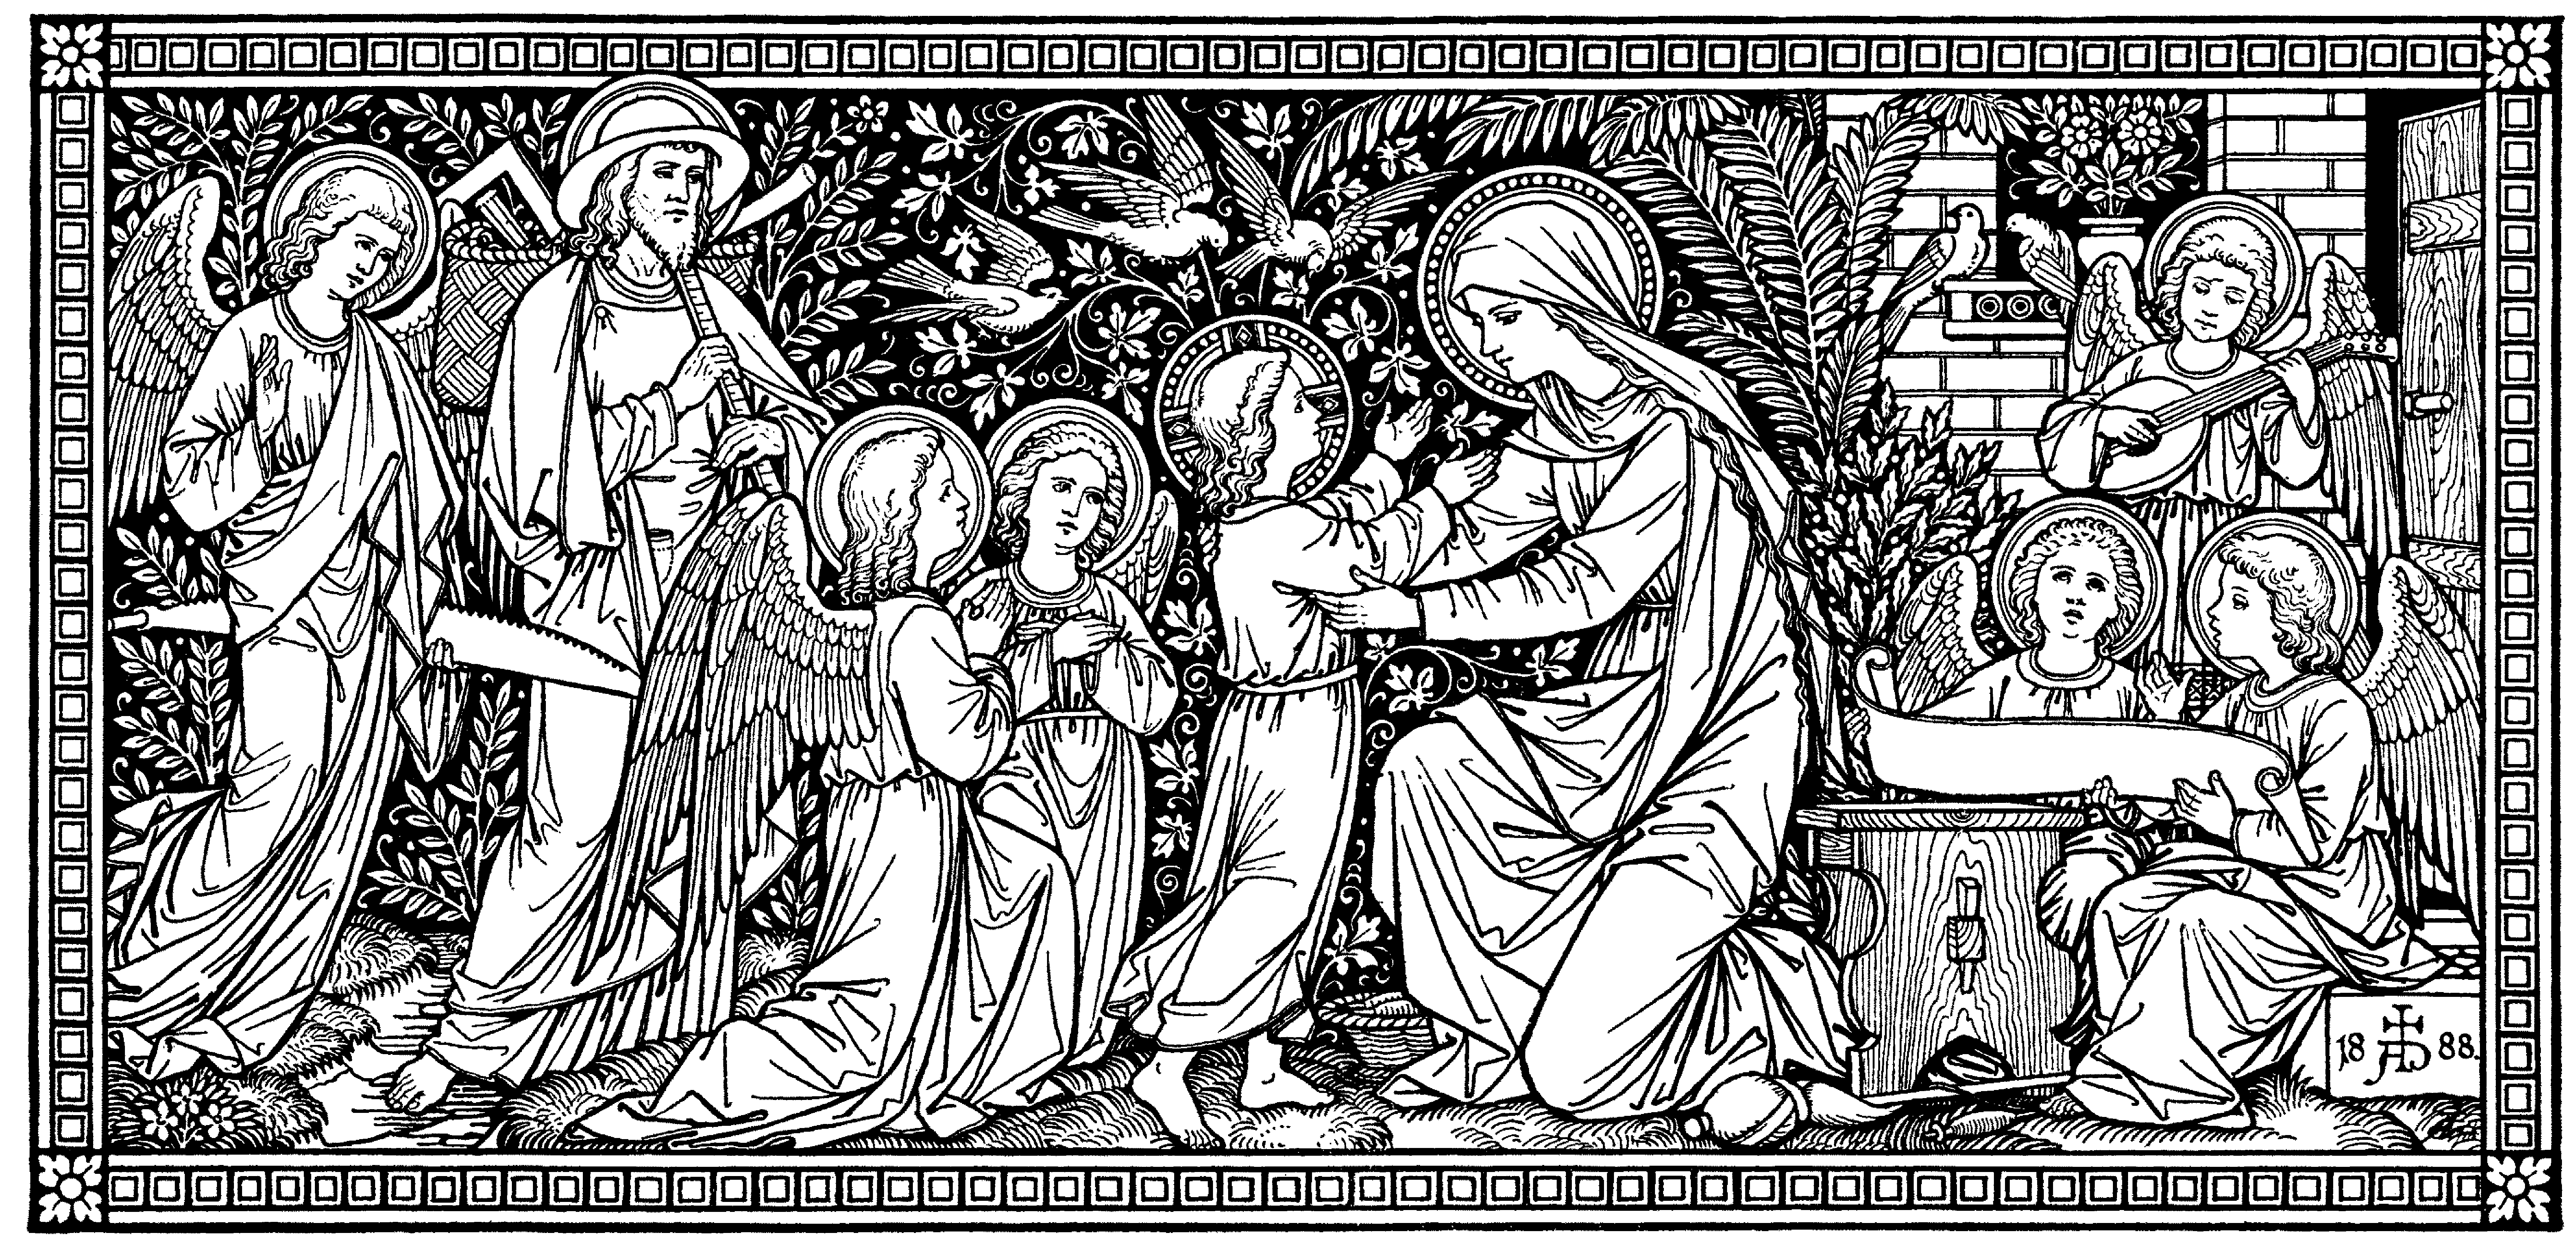
\includegraphics[height=5.5cm]{images/SainteFamille}
\end{center}
\end{document}